%%
%\listfiles
%\documentclass[%
% reprint,%
%secnumarabic,%
% amssymb, amsmath,%
% aip,cha,%
%groupedaddress,%
%frontmatterverbose,
%]{revtex4-1}
\documentclass[twocolumn,amsmath,amssymb,showpacs,pre,nofootinbib,superscriptaddress]{revtex4-1} %,preprint,jcp

\bibstyle{apsrev}
%\usepackage{docs}%
\usepackage{bm}%
\usepackage{graphicx}
%\usepackage{subcaption}
\usepackage{tikz}
\usepackage{color}
\usepackage{xcolor}
\usepackage{physics}
\usepackage[colorlinks=true,linkcolor=blue]{hyperref}%
%\nofiles
\expandafter\ifx\csname package@font\endcsname\relax\else
 \expandafter\expandafter
 \expandafter\usepackage
 \expandafter\expandafter
 \expandafter{\csname package@font\endcsname}%
\fi
\hyphenation{title}
\newcommand{\JH}[1]{\textcolor{blue}{ JH: #1}}

\begin{document}

\definecolor{pyblue}{HTML}{1F77B4}
\definecolor{pyorange}{HTML}{FF7F0C}
\definecolor{pygreen}{HTML}{2CA02C}
\definecolor{pyred}{HTML}{D62728}
\newcommand*\Diff[1]{\mathop{}\!\mathrm{d^#1}}


%\title{Switchable substrates and thin film morphologies}
%\title{Time varying contact angles and thin film morphologies}
\title{Morphologies of thin liquid film dewetting on time-dependent patterned substrates}

\author{S. Zitz}
\email{s.zitz@fz-juelich.de}
 \affiliation{Helmholtz Institute Erlangen-N\"urnberg for Renewable Energy,\\
  Forschungszentrum J\"ulich,\\
  F\"urther Strasse 248, 90429 N\"urnberg, Germany}%
  \affiliation{Department of Chemical and Biological Engineering, Friedrich-Alexander-Universit\"at Erlangen-N\"urnberg, F\"{u}rther Stra{\ss}e 248, 90429 N\"{u}rnberg, Germany}
\author{A. Scagliarini}%
\email{andrea.scagliarini@cnr.it}
 \affiliation{Institute for Applied Mathematics "M. Picone" (IAC), \\
Consiglio Nazionale delle Ricerche (CNR),\\
Via dei Taurini 19, 00185 Rome, Italy}%
\affiliation{INFN, sezione Roma ``Tor Vergata'', via della Ricerca Scientifica 1, 00133 Rome, Italy}
\author{J. Harting}
\email{j.harting@fz-juelich.de}
 \affiliation{Helmholtz Institute Erlangen-N\"urnberg for Renewable Energy,\\
  Forschungszentrum J\"ulich,\\
  F\"urther Strasse 248, 90429 N\"urnberg, Germany}%
 \affiliation{Department of Chemical and Biological Engineering and Department of Physics, Friedrich-Alexander-Universit\"at Erlangen-N\"urnberg, F\"{u}rther Stra{\ss}e 248, 90429 N\"{u}rnberg, Germany}
\date{\today}

\begin{abstract}
We study the dynamics of an unstable thin film deposited on a ``switchable`` substrate.
The substrate is itself subject to a time varying function that affects the contact angle $\theta(\mathbf{x},t)$.
We show that in the case of vanishing time dependence the patterning drives the dewetting morphology and that all fluid is drained into regions of small $\theta(\mathbf{x})$ and thus form droplets.
Interestingly enough with a time varying component to the pattern we are able to stop the droplet fragmentation and create pronounced ligament or rivulet morphologies.
We show that both the numbers of semistable rivulets as well as number of stable droplets can be controlled with the pattern wavelength ($\lambda$).
Finally we explain why the ligaments appear with a simple balance between capillary retraction and dynamic wetting.   
\end{abstract}

\maketitle

\newcommand{\ts}{\textsuperscript}
%\tableofcontents

\section{Introduction}\label{sec:intro}
Wet surfaces and droplets are part of our every-day experience and of several industrial processes,
such as coating, tribology, painting and printing,
to name but a few~\cite{gross1980fluid,szeri2010fluid,DERYCK1998278,doi:10.1146/annurev.fluid.31.1.347,DASILVASOBRINHO19991204,singh2010inkjet,jo2009evaluation}. 
%Being it the droplets condensed in the higher atmosphere and return to the ground as rain or the oil film in a pan during cooking. 
%While this two examples are illustrative there are many industrial applications that build on thin film flows. 
%Among them is the wetting of surfaces to reduce wear or put simply, lubrication~\cite{ReynoldsLubr, gross1980fluid, szeri2010fluid}. 
%Coating surfaces to change their physio-chemical properties is another widely used application~\cite{DERYCK1998278, doi:10.1146/annurev.fluid.31.1.347, DASILVASOBRINHO19991204}.
%On the other hand the need to control droplets is at the heart of many printing processes~\cite{singh2010inkjet, jo2009evaluation}.
Moreover, the continuously growing technological interest for lab-on-a-chip devices~\cite{C6LC00387G,Focke} as well as for
printable electronics~\cite{Kim_2005, Luechinger_2008}, whose efficiency relies crucially on a precise control of material deposition upon dewetting of
liquid films, drew the attention to applications where the substrate is adaptive or switchable, i.e. it is not inert but responds
dynamically to external stimuli or to the evolution of the coating liquid film itself~\cite{doi:10.1126/science.288.5471.1624, doi:10.1246/bcsj.20180076, xin2010reversibly}.
%More recently lab-on-a-chip devices have acquired much attention, to work they require precise droplet or
%film flow on small scales~\cite{stone2004engineering, darhuber2010planar}.
%One possibility for precise control is the local wettability.
%Light switchable substrates~\cite{WANG200718}, therefore substrates that change their wettability based on light illumination, open up a new% way to program this devices. 

Spatial variations of the contact angle are long known and used in previous studies~\cite{PhysRevE.91.023013, Sommers_2006}, time dependency of the contact angle on the other hand is not as well studied~\cite{suman2006dynamics}. 
Switchable substrates are in fact a realization of a time dependent contact angle. 
Using both spatial as well as time dependent variations of the local contact angle leads to interesting phenomena, for example continuously sliding droplets as shown by Grawitter and Stark~\cite{D0SM02082F}.  
Our approach builds on the same idea but our method, see ref~\cite{PhysRevE.100.033313}, allows us to go beyond a single droplet and to simulate the full dewetting transition starting with a thin film and ending with droplets.
We use this to show that a time dependent component of the contact angle alter the dewetting morphology quite substantially.
In the limit of a small time dependency or slow evolution of the contact angle field we qualitatively reproduce the results from Grawitter and Stark, such sliding droplets.
Speeding up the evolution of the contact angle field introduces a morphological transition, which to the understanding of the authors have not been looked at so far.
Therefore the purpose of this manuscript is to increase the understanding of the dewetting process.
Highlighting the fact that a temporal and spatial variation of the contact angle leads to novel morphological structures.
Thus our finding offer a simple way to understand how time periodic switchable substrates could generate novel dewetting morphologies.

The manuscript is outlined as follows:
In section~\ref{sec:method} we discuss the numerical method we use to generate our results and introduce relevant scales.
We then present our results in section~\ref{sec:results}, where we discuss the impact of the time dependency on the contact angle and show that both stability as well as dewetting morphology is affected.
A short summary of our finding and a closing conclusion with outlook is given in section~\ref{sec:sum_conclu}.

\section{Numerical model and simulation details}\label{sec:method}
In order to simulate the dewetting dynamics on patterned, ``switchable'', substrates, we integrate numerically the thin-film equation~\cite{ReynoldsLubr,RevModPhys.69.931,RevModPhys.81.1131} 
\begin{equation}\label{eq:thinfilm}
    \partial_t h(\mathbf{x},t) = \nabla\cdot\left(M_{\delta}(h)\nabla p(\mathbf{x},t)\right),
\end{equation}
by means of a recently developed method, based on a lattice Boltzmann
scheme~\cite{PhysRevE.100.033313,PhysRevE.104.034801}.
Eq.~(\ref{eq:thinfilm}) describes, in a lubrication approximation spirit, the evolution of the height field (film thickness) $h(\mathbf{x},t)$, denoting the location of the liquid/air interface;
the mobility function $M_{\delta}(h)$ depends on the velocity boundary condition at the substrate, parameterized by an effective slip length $\delta$, and reads
\begin{equation}\label{eq:mobility}
  M_{\delta}(h) = \frac{2h^3 + 6\delta h^2 + 3\delta^2h}{6\mu},
\end{equation}  
(which, for $\delta \rightarrow 0$, reduces to the no-slip form $h^3/(3\mu)$),
where $\mu$ is the fluid dynamic viscosity.
The film pressure $p(\mathbf{x},t)$ consists of the sum of the Laplace and disjoining pressures, that is $p(\mathbf{x},t) = -\gamma \nabla^2 h - \Pi$. The disjoining pressure
$\Pi$ can be seen as (minus) the derivative, with respect to the film thickness, of an effective interfacial potential; as such, it contains the information on the
liquid/solid and solid/gas interactions and, hence, on the wettability, which is parameterized in terms of the contact angle, $\theta$ \cite{RevModPhys.81.739, SCHWARTZ1998173}. 
The expression adopted for $\Pi$ is:
\begin{equation}\label{eq:disjoinpressure}
  \Pi(h,\theta) = \frac{2\gamma}{h_{\ast}}(1-\cos(\theta(\mathbf{x},t)))\left[\left(\frac{h_{\ast}}{h}\right)^3 - \left(\frac{h_{\ast}}{h}\right)^2\right],
\end{equation}
where $h_{\ast}$, the height at which the disjoining pressure vanishes, sets the precursor layer thickness.
The time variability of the patterned substrate, then, enters the model precisely through the
disjoining pressure, by making the contact angle space and time dependent, $\theta = \theta(\mathbf{x},t)$.
In particular, the following sinusoidal form is employed:
\begin{equation}\label{eq:sinetheta}
    \theta(\mathbf{x},t) = \theta_0 + \delta\theta\left[\sin\left(\frac{2\pi (x+v_{\theta x}t)}{\lambda}\right)\sin\left(\frac{2\pi (y+v_{\theta y}t)}{\lambda}\right)\right], 
\end{equation}
with $\theta_0 = 20^{\circ}$ and $\delta\theta=10^{\circ}$; the pattern evolves in time as a plane wave.
We choose to fix the velocity direction to one diagonal, i.e.
$\mathbf{v}_{\theta} = (v_{\theta x},v_{\theta y}) = v_{\theta}(1/\sqrt{2},1/\sqrt{2})$.
Notice that, since a typical velocity is such that $v_{\theta} \Delta t \ll \Delta x$ (in one time step the wave would travel
a distance much smaller than a lattice spacing), the time update must be interpreted in an integer part sense, that is
the pattern is shifted by one $\Delta x$ every $1/v_{\theta x}$ time steps (and equivalently in the $y$-direction).
%The second pattern is a triangle wave which accounts for a different kind of pattern gradient.
%To the best of our knowledge contact angles can not be tuned precise enough to match a sinusoidal wave on %the scales we are interested in.
%Therefore we assume that a triangle wave with a linear gradient is more likely accessable in experiments, %thus $\theta_2$ is given as
%\begin{equation}\label{eq:triangle_wave}
%\begin{split}
%    \theta_2(x,y) &= \theta_0 + \\ &\frac{2\delta\theta}{\pi}\left[\sin^{-1}\left(\sin\left(\frac{2\pi x}{%\lambda}\right)\right)\sin^{-1}\left(\sin\left(\frac{2\pi y}{\lambda}\right)\right)\right].
%    \end{split}
%\end{equation}
%Both patterns create a contact angle distribution with values within the interval $[10^{\circ}, 30^{\circ}%]$ and by definition they are time independent.
%To have a time dependency we simply shift the pattern in a periodic manner, such that
%\begin{equation}\label{eq:theta_shift}
%    \theta(\mathbf{x},t+T) = \theta(\mathbf{x}-\mathbf{1}, t), 
%\end{equation}
%with $T$ being an arbitrary integer number of lattice Boltzmann time steps.
Hereafter, lengths will be meant expressed in units of the
mean film height, $h_0$ (which is constant in time, due to mass conservation) and pattern wavelength $\lambda$, whereas the charactestic
time scale is set by:
\begin{equation}\label{eq:t0}
t_0 = \frac{3\mu}{\gamma h_0^3 q_0^4},
\end{equation}
where $\gamma$ is the surface tension
(the numerical values, in lattice Boltzmann units, are set to $\gamma = 0.01$ and $\mu=0.167$).
The thus defined $t_0$ is the inverse growth rate of the most unstable mode (of wavenumber $q_0$)
of a spinodally dewetting film (on a homogeneous substrate) \cite{Mecke_2005,PhysRevE.100.023108};
in our heterogeneous case, we define the wavenumber $q_0$ as 
$q_0^2=\frac{1}{2\gamma}\frac{\partial \Pi(h,\theta)}{\partial h}(h=h_0,\theta=\theta_0+\delta \theta)$.
At this point, a reference velocity can also be constructed as
\begin{equation}\label{eq:v0}
v_0 \equiv \frac{\lambda}{t_0}.
\end{equation}
%Due to convenience we attribute a velocity to the pattern which is the shift distance divided by the stepp%ing time
%\begin{equation}\label{eq:pattern_speed}
%    v_{\theta} = \frac{\sqrt{2}}{T}.
%\end{equation}
%Since this velocity as well as the choice of $T$ is arbitrary we define a characteristic velocity $v_0$ si%milar to Eqs.~(\ref{eq:q0_and_t0}) as
%\begin{equation}\label{eq:normvel}
%    v_0 = \frac{\lambda}{t_0(\theta)},
%\end{equation}
%where we use the wavelength $\lambda$ as a characteristic distance and $t_0(30^{\circ})$ as a characterist%ic time scale.
%Important to note is that $t_0$ is sensitive to the contact angle, and decreases with increasing angle.
\begin{figure}
    \centering
    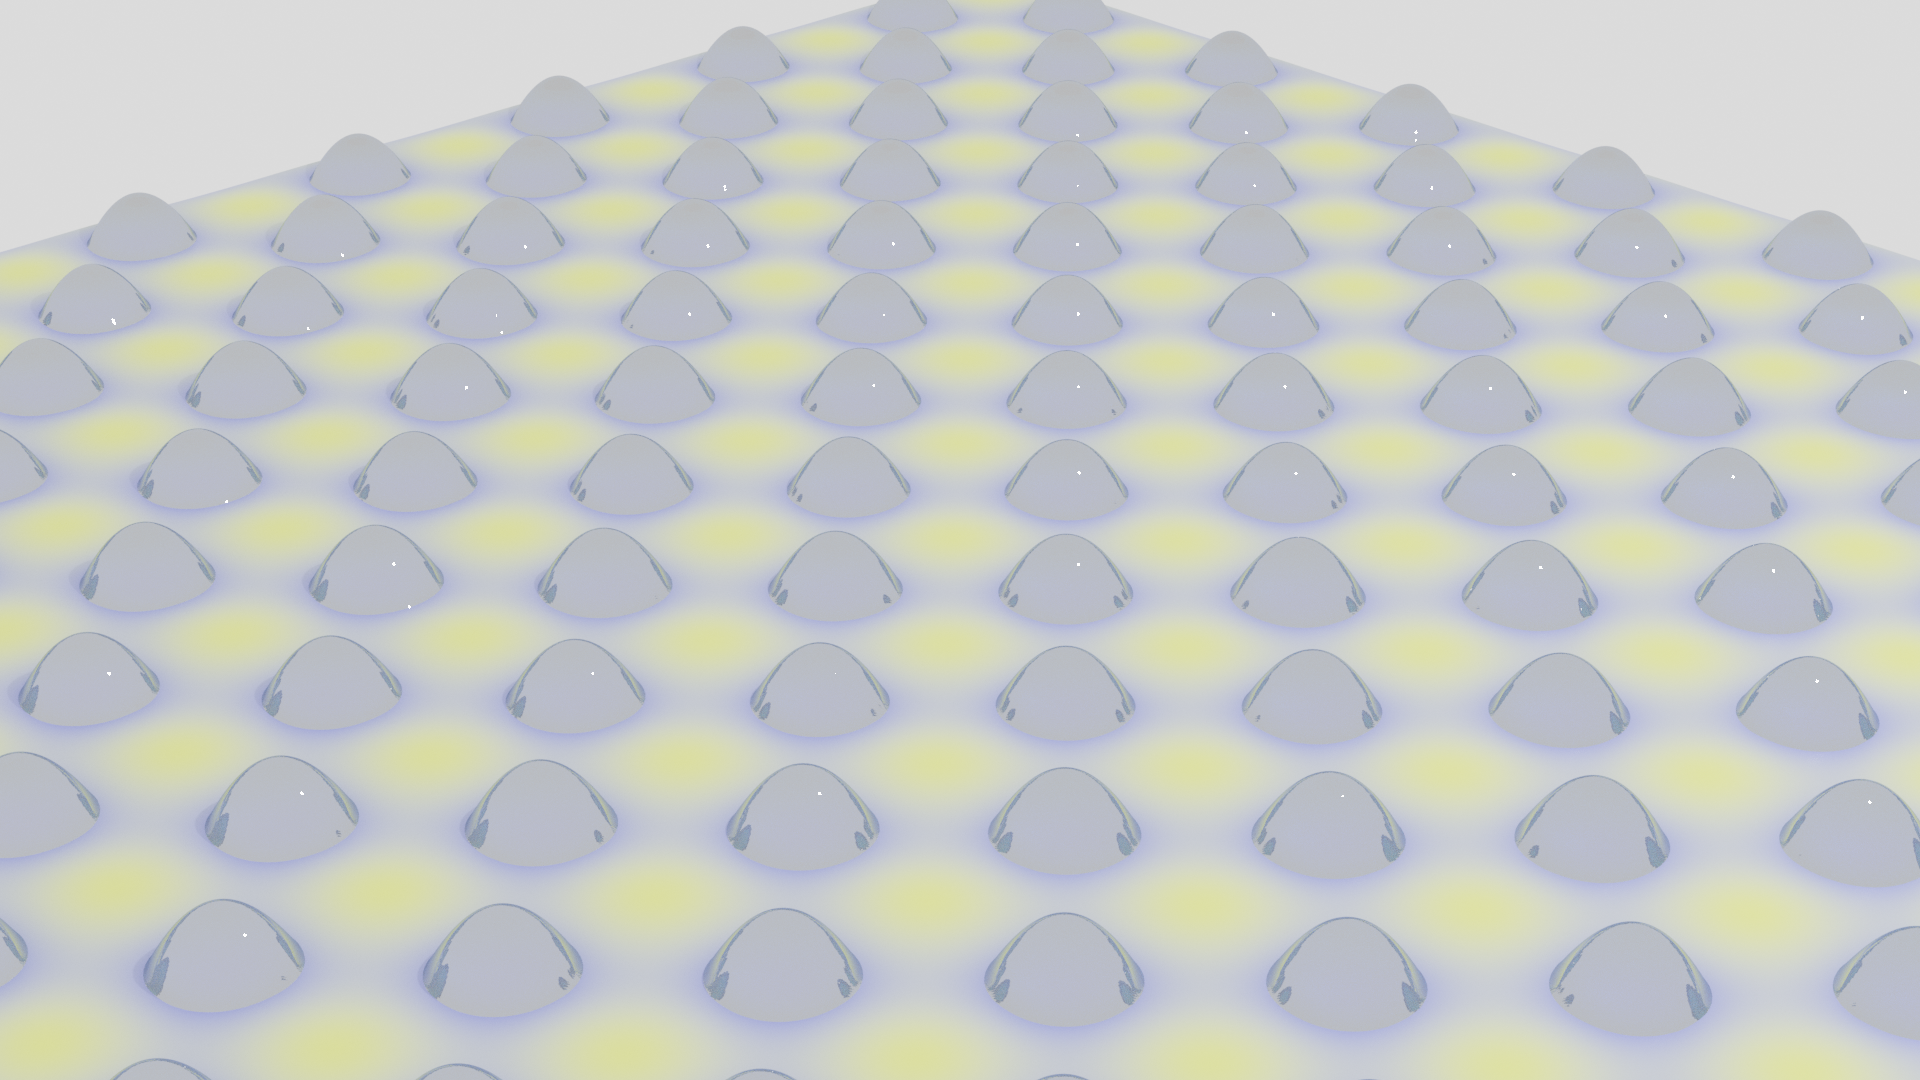
\includegraphics[width=0.45\textwidth]{Figures/No_vel_render.png}
    \caption{Rendered image of the film on the stationary contact angle pattern at late times ($t > 20t_0$).
    The contact angle field is color coded, areas where the angle is small (high) are shown in blue (yellow).}
    \label{fig:handtheta}
\end{figure}
%As outlined in Sec.~\ref{subsec:LBM} we simulate the evolution of the thin film with a lattice Boltzmann m%ethod.
All our simulations are run on a bi-periodic square domain of size $L \times L$ with $L = 512$.
%Having this value of $\mu$ leaves us with a relaxation time $\tau = 1$.
To regularize the contact line divergence~\cite{huh1971hydrodynamic} we use a precursor layer thickness
$h_{\ast}=0.07$ and and a slip length $\delta = 1$
(see Eqs.~(\ref{eq:mobility})-(\ref{eq:disjoinpressure})). 
% With this choice of parameters we are almost able simulate a no-slip boundary condition.
%As for our disjoining pressure potential, see Eq.~(\ref{eq:disjoinpressure}), we use the power pair
%$n=3, m=2$ and $h_{\ast} = 0.07$.
%Inserting this quantities into Eq.~(\ref{eq:q0_and_t0}) with $h_0 = 1$ yields $q_0^2(30^{\circ}) \approx 1%.68\cdot10^{-2}$ as well as $t_0(30^{\circ}) \approx 177000\Delta t$ which gives us a first glimpse into r%elevant length and time scales.
The liquid film is initiliazed with a height field slightly perturbed around the mean valued $h_0=1$, i.e.:
\begin{equation}\label{eq:hinitial}
    h(\mathbf{x},0) = h_0 \left[1 + 0.1 \left(\sin\left(\frac{2\pi x}{L}\right)\sin\left(\frac{2\pi y}{L}\right)\right)\right].
\end{equation}
Various wavelengths, in the range $\lambda \in [L/9, L]$, and velocities, $v_{\theta} \in [0.1, 10]v_0$,
are considered for the wettability pattern, Eq.~(\ref{eq:sinetheta}). 
%We proceed as follows, first we simulate the dewetting on a given pattern either sinusoidal- or triangular% with  without a time dependency in $\theta$.
In Fig.~\ref{fig:handtheta} we show $h(\mathbf{x},t)$ (droplets) and $\theta(\mathbf{x})$ (color coded) for $v_{\theta} = 0$ (i.e. the stationary case) and $\lambda = L/2$, in late stages of dewetting.
As expected, droplets form in regions of small contact angles (blue) while the regions of high contact angles (yellow) dewet.
%In subsequent simulations we iterate through , see Eq.~(\ref{eq:normvel}) .  
% Based on $v_{\theta}$ we can modify the morphology of the dewetting film, in both the intermediate transition regime as well as the late time state.

\section{Results}\label{sec:results}

\subsection{Rupture times}\label{subsec:rupture}

We want to study how the rupture times depend on the parameters characterising the wettability pattern, namely the contact angle
wavelength, $\lambda$, and wave speed, $v_{\theta}$.
The film rupture time, $\tau_r$, is defined as the least $t$ such that $\{\exists\mathbf{x}: h(\mathbf{x},\tau_r)=h_{\ast}\}$ (that is, when the
free surface touches the substrate).
%Taking another look at Fig.~\ref{fig:deltah_v0_sine} reveals that the three wavelengths rupture at different times $\tau_r$.
%The most important values for $\tau_r$ can be found in Tab.~\ref{tab:rup_times}.
In Fig.~\ref{fig:model_rt} we report the rupture times, as a function of the wavelength, for the stationary pattern ($v_{\theta}=0$) and
for $v_{\theta}=10 v_0$. We observe that, in both cases, $\tau_r$ grows $\lambda$.
%Thus smaller values of $\lambda$ lead to an earlier rupture time.
%Which can be explained with a mismatch of length scales.
This fact can be explained, qualitatively, as follows.
There is a length scale set by Eq.~(\ref{eq:disjoinpressure}) ($\lambda_0 = 2\pi/q_0$) and one that we introduce with the substrates wavelength $\lambda$.
\begin{figure}
    \centering
    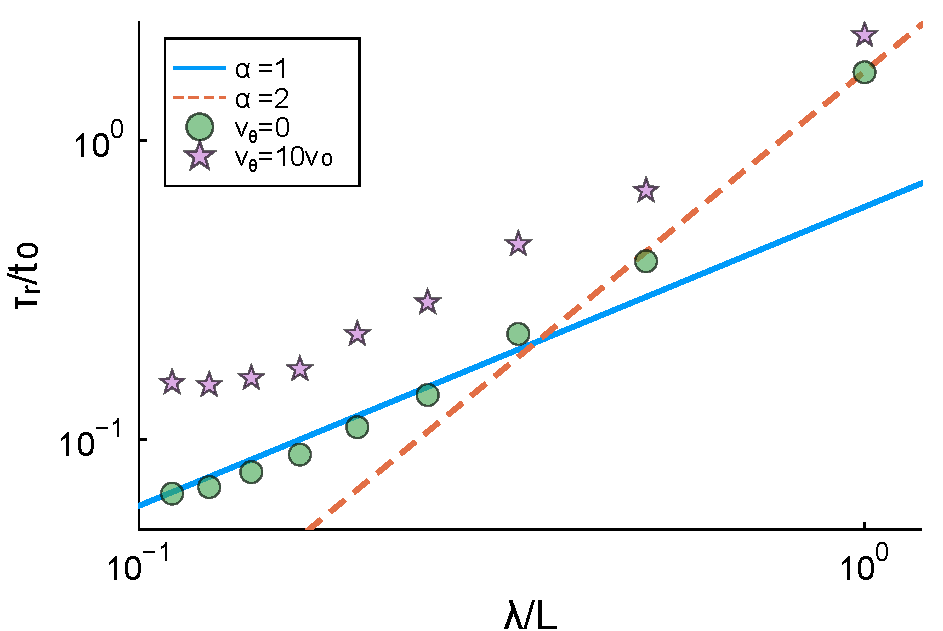
\includegraphics[width=0.48\textwidth]{Figures/Rupture_times_over_lambda_with_powerlaw.pdf}
    \caption{Distribution of rupture times $\tau_r$ normalized by $t_0$ for different pattern wavelengths $\lambda$.
    The bullets, stars correspond to data from our simulations with $v_{\theta} = 0, 10v_0$.
    The full blue and dashed orange line are generated using $f(x) = a~x^{\alpha}$, with $a=0.6,1.5$ respectively.
    }
    \label{fig:model_rt}
\end{figure}
Taking this into account we can model the rupture times for the stationary pattern with
\begin{equation}\label{eq:model_tr}
    \frac{\tau_r}{t_0} = \frac{1}{2\pi}\frac{L}{\lambda_0 i^D}\approx \xi\frac{\lambda}{\lambda_0},    
\end{equation}
where $i$ is the wavenumber of the substrates pattern ($\lambda = L/i$) and $D$ is the dimension, thus $D=2$.

Interestingly, the behaviour of $\tau_r$ vs $\lambda$ remains qualitatively the same also for the
time-dependent case, $v_{\theta} = 0.1v_0$, reported in Fig.~\ref{fig:model_rt} as blue squares.
%as the difference of rupture times between these two simulations is negligible,
%see Tab.~\ref{tab:rup_times}.
Nevertheless, larger $v_{\theta}$ introduce a shift towards longer rupture times, i.e. fast wettability
waves tend to stabilise the film.
%Next we look into the affects of the pattern velocity on the structure formation after the first ruptures.

\subsection{Morphologies}\label{subsec:morpho}
We now look into the long time dynamics, focusing, in particular on the characterisation of the
dewetting morphologies and how they are affected by the speed of the wettability wave.

\subsubsection{Stationary pattern}\label{subsec:no_vtheta}
%Starting with Eq.~(\ref{eq:hinitial}) we have by definition an unstable film that will rupture.
%This can be easily seen by the fact that the initial perturbation has the smallest possible wavenumber, $q(t=0)=1/L$.
%Taking into account the addition of the wettability gradient we know that fluid will accumulate in regions of high surface energies or
%small contact angles and flow away from regions of high contact angle.
%An illustrative results of this effect is shown in Fig.~\ref{fig:handtheta}, where all droplets are present in a region of
%small contact angles.
\begin{figure}
    \centering
    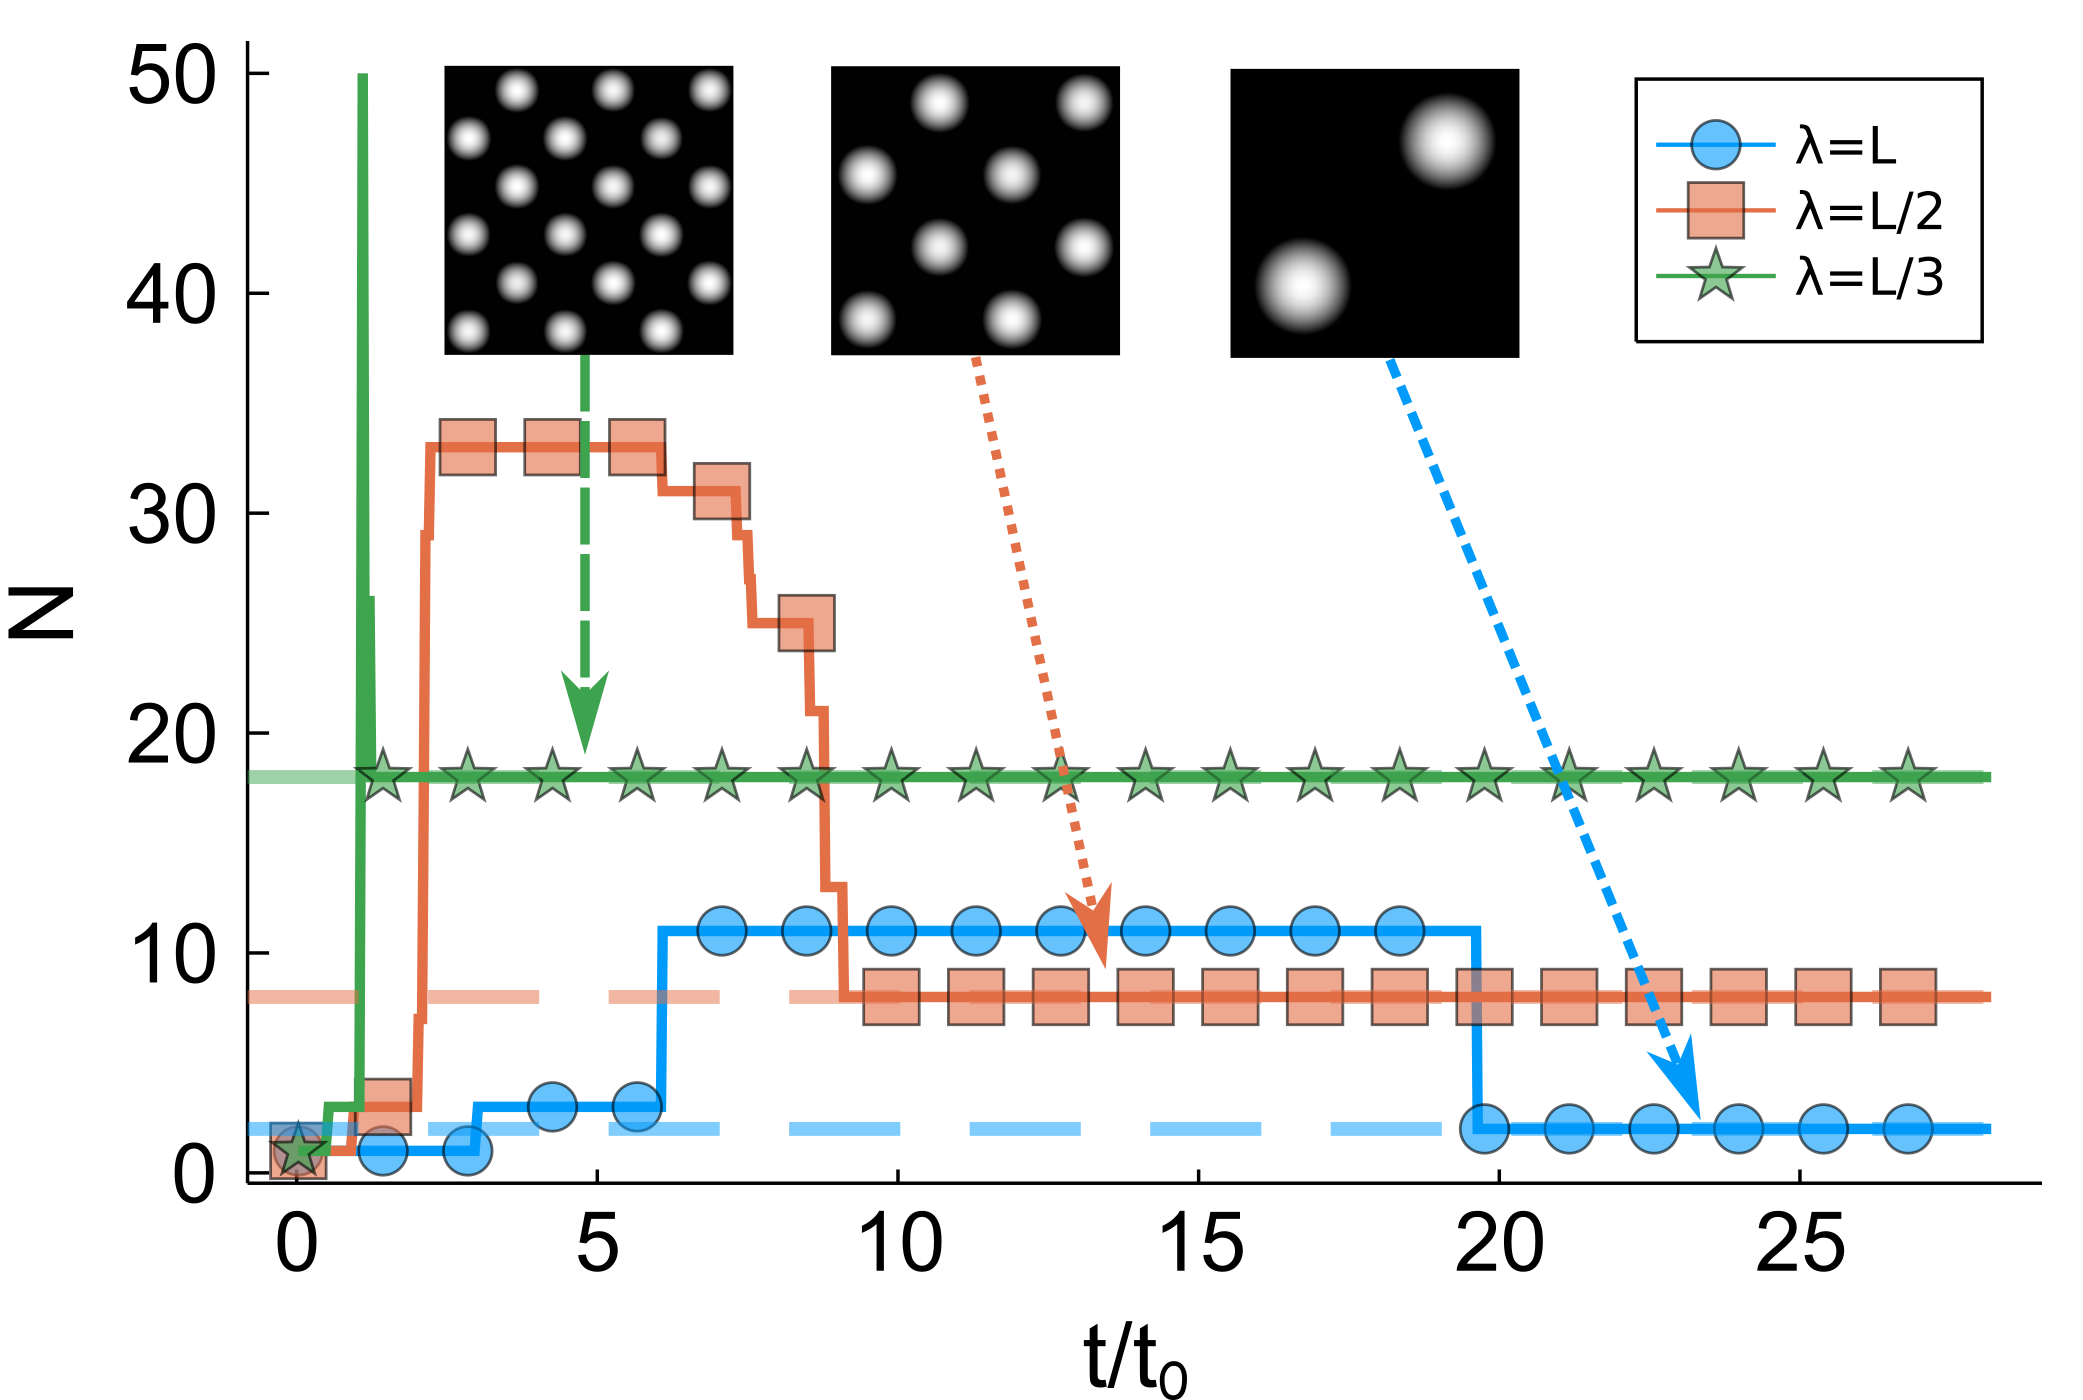
\includegraphics[width=0.4\textwidth]{Figures/Clusters_novel_sine_picutres.png}
    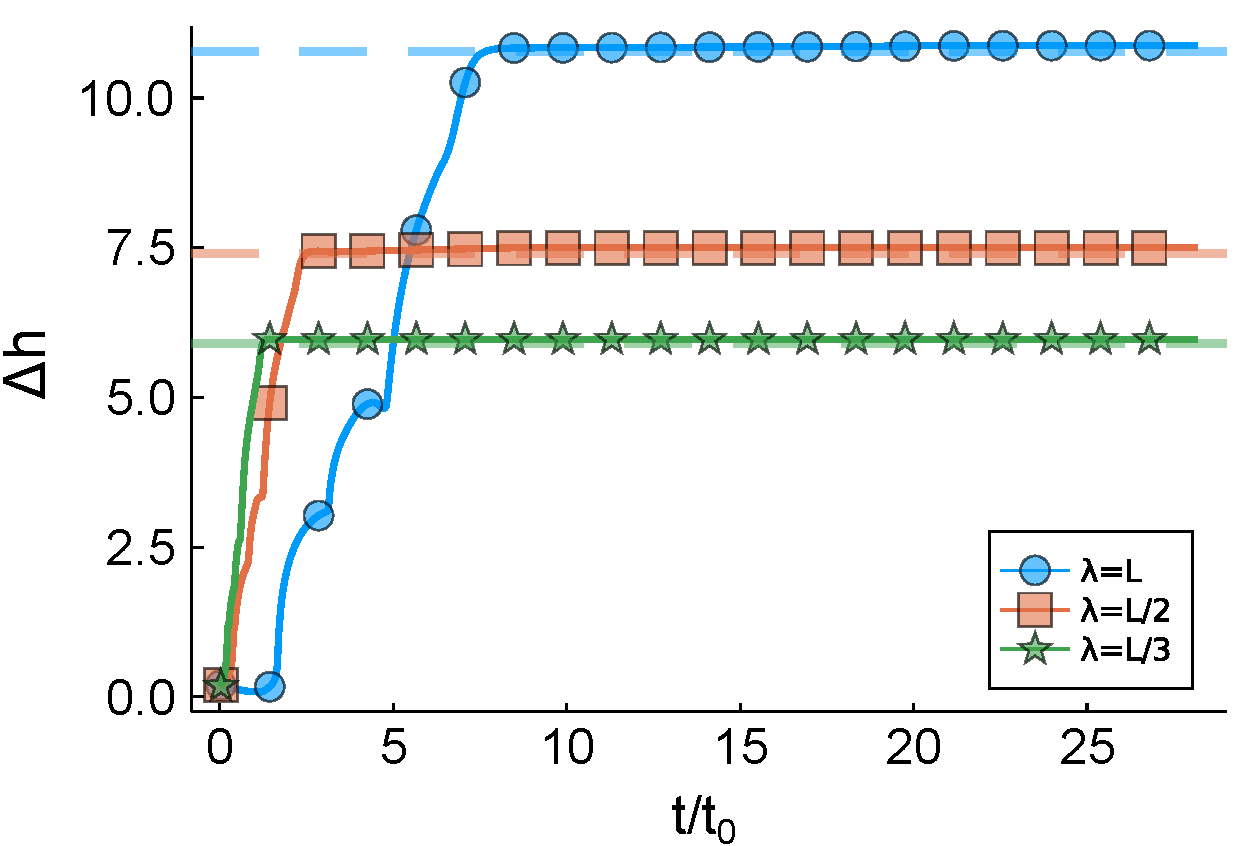
\includegraphics[width=0.45\textwidth]{Figures/delta_h_v0_sin_with_dash.pdf}
    \caption{TOP PANEL. Number of droplets, $N$, as a function of time, generated during the dewetting process on the patterned substrate
      given by Eq.~(\ref{eq:sinetheta}), with $v_{\theta}=0$ and $\lambda=L$ (blue circles), $\lambda=L/2$ (orange squares) and
      $\lambda=L/3$ (green stars). The three horizontal dashed lines indicate the number of minima of (\ref{eq:sinetheta}),
      which is $2\left(\frac{L}{\lambda}\right)^2$. In the insets, we show shanpshots of the stationary droplet state as a grayscale image
      of the film thickness $h(\mathbf{x},t_{\infty})$.
      BOTTOM PANEL. Evolution of $\Delta h$ with time.
      Different symbols and colors represent different pattern wavelengths.
      Dashed lines indicate solutions to the cap height $h_d$ given the volume is split equally among the droplets,
      see Eq.~(\ref{eq:height_guess}).}
    \label{fig:clusters_v0_sine}
\end{figure}
%This is in fact a consistency check of our simulations.
On the stationary substrate, after rupture all the fluid accumulates in droplets centered at contact angle minima.
Consequently, as we see from Fig.~\ref{fig:clusters_v0_sine} where we plot the number of droplets, $N$, in time, 
in the steady state ($t \gg t_0$) such number attains the value $N_{\infty} = 2(L/\lambda)^2$
(which equals the minima of (\ref{eq:sinetheta}), for $v_{\theta}=0$).
%We expect that in case of $v_{\theta} = 0$ all fluid accumulates in droplets inside the contact angle minima.
%While there are only two minima for $\lambda = L$ there are eight and eighteen minima for $\lambda = L/2$ and $\lambda = L/3$ respectively.
%This can be easily checked with a cluster analysis of the film thickness $h(\mathbf{x},t)$ which
%we shown in Fig.~\ref{fig:clusters_v0_sine}.
%The height $h(\mathbf{x},t_{\infty})$ is displayed as grayscale images and is linked to stationary state.
%Theoretically we expect therefor two, eight and eighteen clusters (droplets) which we mark with a vertical
%dashed line in the respective color.
%These values are consistent with our simulations.
Notice that the number of clusters converges faster for smaller pattern wavelengths, in line with the observation, reported
and justified in the previous section, that the characteristic dewetting time decreases with the wavelength.\\
%To some extend this is expected as the distance between contact angle minima is shorter for smaller wavelengths.

Another quantity that is easily accessible and helps to check the consistency of our simulations is the height of the droplets $h_d$.
Given that all the fluid is collected inside the droplets we can make an assumption of the droplets height based on its volume $V_d$  and contact angle $\theta_d$ 
\begin{equation}\label{eq:height_guess}
    h_d(V_d, \theta_d) = \left(\frac{3V_d(1-\cos(\theta_d))}{\pi(2+\cos(\theta_d))}\right)^{\frac{1}{3}},
\end{equation}
where we implicitly assume that all our droplets have a spherical cap shape.
Since our method does not allow $h=0$ we measure the droplets height as~\cite{PhysRevE.100.033313}
\begin{equation}\label{eq:delta_h_measure}
    \Delta h(t) = \max_{\mathbf{x}}\{h(\mathbf{x},t)\} - \min_{\mathbf{x}}\{h(\mathbf{x},t)\}.
\end{equation}
Counting the minima in $\theta(\mathbf{x})$ for the different wavelengths $\lambda$ allows to calculate the volume of a single droplet, see Fig.~\ref{fig:clusters_v0_sine}.
Since the film dewets regions of high contact angle values we can safely assume that $\theta_d < 20^{\circ}$.
%\begin{figure}
%    \centering
%    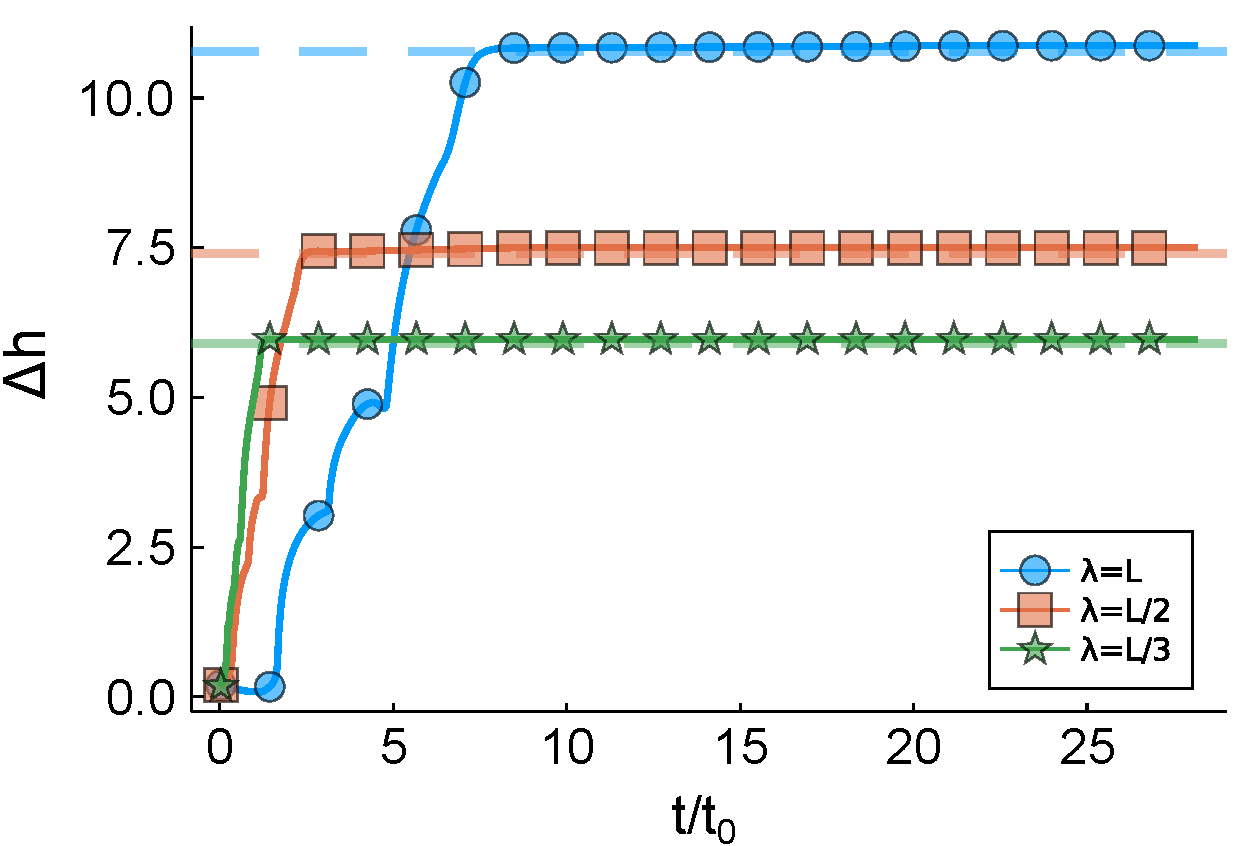
\includegraphics[width=0.48\textwidth]{Figures/delta_h_v0_sin_with_dash.pdf}
%    \caption{Evolution of $\Delta h$ with time.
%    Different symbols and colors represent different pattern wavelengths.
%    Dashed lines indicate solutions to the cap height $h_d$ given the volume is split equally among the droplets,
%    see Eq.~(\ref{eq:height_guess}).}
%    \label{fig:deltah_v0_sine}
%\end{figure}
Measuring the height of the droplets is done in the lower panel of Fig.~\ref{fig:clusters_v0_sine}, where $\Delta h$ is the maximal difference in film thickness which is equivalent to the droplet height $h_d$.
Focusing on the late time behaviour ($t > 10t_0$) we identify plateauing values. 
Since the pattern is a continuous functions, see Eq.~(\ref{eq:sinetheta}), we are left with some degree of freedom for the theoretical $\theta_d$ values. 
As a guide to the eye we introduce three dashed lines.
The dashed lines are calculated using Eq.~(\ref{eq:height_guess}) with $V_d = (V/N_{\infty})$ and $\theta_d = (14^{\circ}, 16^{\circ}, 17^{\circ})$ for $\lambda=(L,L/2,L/3)$ respectively.
These fit values for $\theta_d$ agree well with the stationary droplet state of our simulations.
Thus we are fairly confident that our droplet states and thus the simulations capturing the correct physical state.

%\subsection{Stability}\label{subsec:time_dep_theta}
%\begin{table}[h!]
%  \begin{center}
%    \begin{tabular}{c|c|c|c}
%      \textbf{Pattern} & \textbf{Wavelength} & \textbf{Velocity } & \textbf{Rupture time}\\
%      $\theta(\mathbf{x})$ & $\lambda$ & $v/v_0 $ & $\tau_r/t_0$ \\
%      \hline
%      $\theta_1$ & L & 0 & 1.69\\
%      $\theta_1$ & L & 0.1 & 1.72\\
%      $\theta_1$ & L & 1 & 2.34\\
%      $\theta_1$ & L & 10 & 2.25\\
%      $\theta_1$ & L/2 & 0 & 0.39\\
%      $\theta_1$ & L/2 & 0.1 & 0.39\\
%      $\theta_1$ & L/2 & 1 & 0.59\\
%      $\theta_1$ & L/2 & 10 & 0.68\\
%      $\theta_1$ & L/3 & 0 & 0.23\\
%      $\theta_1$ & L/3 & 0.1 & 0.23\\
%      $\theta_1$ & L/3 & 1 & 0.25\\
%      $\theta_1$ & L/3 & 10 & 0.45\\
%      $\theta_2$ & L & 0 & 1.01\\
%      $\theta_2$ & L & 0.1 & 1.18\\
%      $\theta_2$ & L & 1 & 1.32\\
%      $\theta_2$ & L & 10 & 1.38\\
%      $\theta_2$ & L/2 & 0 & 0.48\\
%      $\theta_2$ & L/2 & 0.1 & 0.48\\
%      $\theta_2$ & L/2 & 1 & 0.7\\
%      $\theta_2$ & L/2 & 10 & 0.76\\
%      $\theta_2$ & L/3 & 0 & 0.39\\
%      $\theta_2$ & L/3 & 0.1 & 0.42\\
%      $\theta_2$ & L/3 & 1 & 0.68\\
%      $\theta_2$ & L/3 & 10 & 0.76\\
%    \end{tabular}
%    \caption{Rupture time values for different pattern wavelengths $\lambda$ and different substrate velocities $v_{\theta}$.
%    Due to sampling we have a systematic error of 0.03 in the rupture times $\tau_r$.}
%    \label{tab:rup_times}
%  \end{center}
%\end{table}

\subsubsection{Time-dependent pattern}\label{subsec:timedep}
Dewetting morphology is a rather broad topic~\cite{becker2003complex, RevModPhys.81.739, PhysRevLett.99.114503, craster2009dynamics, doi:10.1146/annurev-fluid-011212-140734, alizadeh_pahlavan_cueto-felgueroso_hosoi_mckinley_juanes_2018}, however we know that a simple patterned substrate will ultimately yield droplets in region of small contact angle and is likely to rupture in regions of high contact angle, as shown in Fig.~\ref{fig:handtheta}.
This is indeed what we observe for the simulation without pattern velocity ($v_{\theta} = 0$).
\begin{figure}
    \centering
    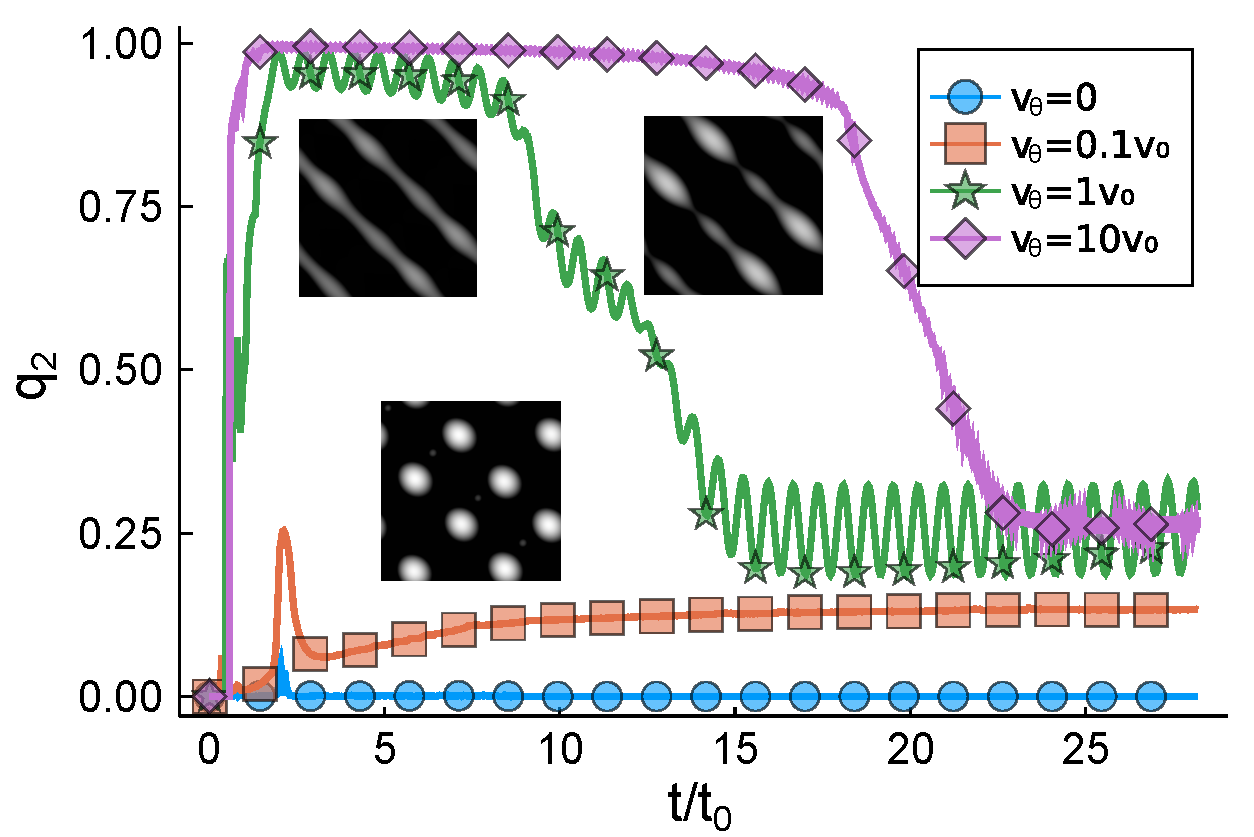
\includegraphics[width=0.48\textwidth]{Figures/q_2_different_v.pdf}
    \caption{Structure analysis of the pattern $\theta_1,~\lambda=L/2$ using the Minkowski structure metrics (MSM). 
    The dipole metric $q_2$ is plotted for different pattern velocities $v_{\theta}$, displayed with different colors and symbols.
    In grayscale we supply the film thickness that is associated with the $q_2$ values.
    }
    \label{fig:msm_q2}
\end{figure}
Increasing the pattern velocity $v_{\theta} > 0$ does affect the dewetting morphology quite substantially.
Having $v_{\theta} = 0.1 v_0$ we are still observing the formation of droplets, similar to $v_{\theta} = 0$ but instead of being stationary these droplets, depending on their mass, are transported with the contact angle minima.
A somewhat similar behaviour was recently described by Grawitter and Stark~\cite{D0SM02082F} where they have used a boundary integral method to simulate a droplet on a moving wettability step.

If the pattern velocity is further increased $v_{\theta} > 0.1 v_0$ we observe a transition towards ligament or rivulet like structures.
These structures are aligned with the update direction of the contact angle field, see Eq.~(\ref{eq:sinetheta}). 
Thus if
\begin{equation*}
    \theta(x,y,t+T) = \theta(x-1, y, t),    
\end{equation*}
ligaments form in x direction.
These ligaments are sensitive to $\lambda$, or more precisely to the contact angle minima since they attract fluid.
To classify the morphological differences in respect to $v_{\theta}$ we make use of \textbf{papaya2}~\cite{Schaller2020}.

We use the film thickness as input and compute different morphological metrics.
Among the most interesting ones are the Minkowski structure metrics (MSM) $q_s$.
They can be calculated using~\cite{doi:10.1063/1.4774084}
\begin{equation}
    q_s(K) = \frac{|\psi_s(K)|}{\psi_0(K)}, 
\end{equation}
where $K$ is the body to we extract morphological information from and $\psi_s$ are the irreducible Minskovski tensors (IMT)
\begin{equation}
    \psi_s(K) = \int_{0}^{2\pi}e^{is\phi}\rho_K(\phi) \dd\phi = \sum_{k=-\infty}^{\infty} L_k e^{is\phi_k},
\end{equation}
with $L_k$ being the set of normal vectors of the body $K$.
Within the various $q_s$ we are particularly interested in the dipole one $q_2$. 
With $q_2$ we can clearly distinguish between a droplet and a ligament structure, as we expect a much larger $q_2$ value for the later one which is what we see in Fig.~\ref{fig:msm_q2}.
Our simulations with $\lambda = L/2$ show a clear difference between $v_{\theta} \leq 0.1v_0$ and $v_{\theta}>0.1v_0$  in $q_2$.
Interestingly the $q_2$ values for $v_{\theta} = 0.1v_0$ are always larger than those of $v_{\theta} = 0$.
Even the smallest pattern velocity introduces a measurable deformation of the spherical cap shape.

\begin{figure}
    \centering
    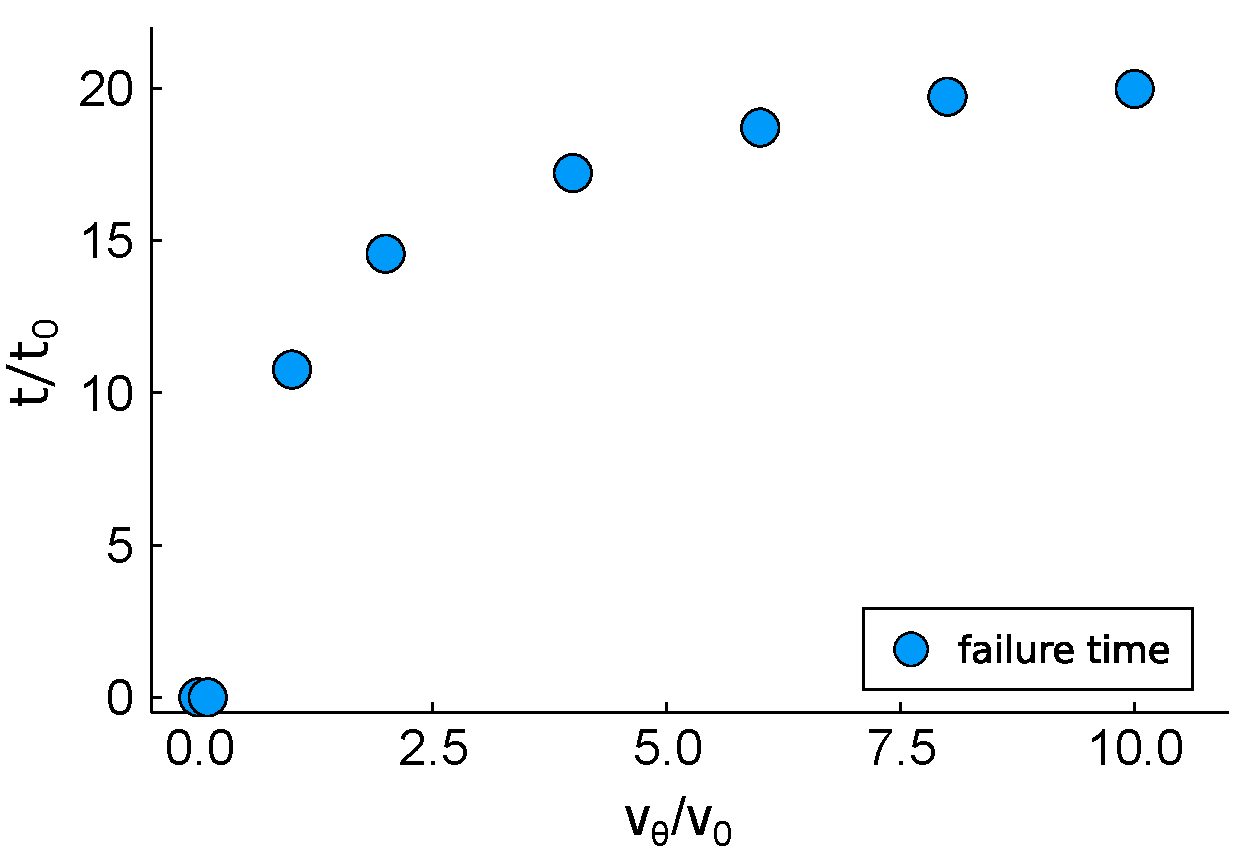
\includegraphics[width=0.45\textwidth]{Figures/stab_lig_lam2_v2.pdf}
    \caption{Measurement of the stability of the ligaments in terms of $q_2$.
    The failure time is defined as the time when the value of $q_2$ is below a threshold value.
    If no ligaments formed at all, the failure time is set to 0.
    }
    \label{fig:stab_ligs_lam2}
\end{figure}
Moving the contact angle field faster creates metastable ligament states.
Metastable because this ligaments will eventually break and separate into droplets.
This is indicated in Fig.~\ref{fig:msm_q2} by the dip in $q_2$ for $v_{\theta} = 1, 10 v_0$ (green and violet curve).
The breakup is actually due to the varicose mode of the ligament~\cite{doi:10.1063/1.3211248, PhysRevE.77.061605}.
Interestingly the wavelength of this varicose mode is $\approx\lambda$ and therefore we only observe $N_{\infty}/2$ droplets after breakup.
An analysis of the stability of these ligaments can be found in Fig.~\ref{fig:stab_ligs_lam2}.
Two things can be seen in this plot, first being the fact that ligaments only form for $v_{\theta} > 0.1$.
On the other hand a saturation happens for large $v_{\theta}$ values. 
Meaning we do not observe an increase in the lifetime of a ligament for $v_{\theta} > 10$.
% One possibility for that behaviour is that due to fast update of the pattern the film only experiences a singular effective contact angle value.
Besides the fact that only $N_{\infty}/2$ droplets are formed after ligament failure we observe on top a different dynamic than the ones on slow or no pattern velocity.   
Instead of a continuous motion with the pattern the remnants of the ligament are in an oscillating pumping state.
In this state the droplets are to slow to follow the pattern, which leads to cycle of deformation and retraction driven by the pattern (see sup. material).
This behaviour is clearly captured by Fig.~\ref{fig:msm_q2}, see e.g. the green curve for $t > 15t_0$.
Nevertheless the formation of ligaments in the first place can be explained with a few relative simple assumptions.

This problem is associated with two time scales, first being $t_0(\theta)$ the time scale of the dewetting thin film, see Eq.~(\ref{eq:t0}).
After the rupture we identify another time scale, the capillary time scale $\tau_{\text{Ca}}$ that drives the rims away from the holes~\cite{Edwardse1600183},
\begin{equation}\label{eq:cap_time}
    \tau_{\text{Ca}} = \frac{9\mu l_0}{\gamma \theta^3(\mathbf{x})},
\end{equation}
where  $l_0$ is a characteristic length scale of the problem, we use $\lambda/2$ as two rims can travel at most $\lambda/2$ before they merge.
Knowing this time scales allows us to introduce characteristic velocities.
One of these two is $v_0$ which is given by Eq.~(\ref{eq:v0}) and used to normalize $v_{\theta}$.
The other one is set by $\tau_{\text{Ca}}$ and reads
\begin{equation}\label{eq:cap_speed}
    U_{Ca} =\frac{l_0}{\tau_{\text{Ca}}} = \frac{\gamma}{9\mu} \theta^3(\mathbf{x}), 
\end{equation}
where $U_{\text{Ca}}$ is the capillary speed.
The argument is as follows, if $U_{\text{Ca}}$ is large as compared to $v_{\theta}$ than the film retraction is faster than the transport due to the contact angle field and thus droplets from.
Which explains the cases of $v_{\theta} = 0$ and  $v_{\theta} = 0.1v_0$.
On the other hand if $v_{\theta}$ is larger than $U_{\text{Ca}}$ than the retracting film has to little time to form droplets and ends up in the metastable ligament state.
Taking a look at our simulations with $v_{\theta} = 1v_0$ and $v_{\theta} =  10v_0$ we clearly observe ligament states.

In fact the ratio 
\begin{equation}\label{eq:vel_ratio}
    \Gamma = \frac{v_{\theta}}{U_{\text{Ca}}} = \frac{3\lambda \chi h_0^3 q_0^4}{\Theta^3}, 
\end{equation}
where $\Theta = max(\theta(\mathbf{x}))$ and $v_{\theta} = \chi v_0$, allows to classify the dewetting morphology on a time and space dependent substrate pattern. 
% as
% \begin{equation}\label{eq:classify}
%     \Gamma~\begin{cases}
%     < 1\qquad ... \text{droplets} \\
%     > 1\qquad ... \text{ligaments} 
%     \end{cases}.
% \end{equation}
% This explains in fact what we observe and holds true independent of the wettability gradient, i.e. $\theta_1, \theta_2$.

Therefore by varying either $\chi$ or $\lambda$ for a fixed $\Theta$ one can change the intermediate dewetting morphology according to Eq.~(\ref{eq:vel_ratio}).
Interestingly but not surprising is the fact that the fluid transport is larger for $\Gamma > 1$ than for $\Gamma < 1$.

\section{Summary and Conclusions}\label{sec:sum_conclu}
To summarize, we have shown numerical simulations of a dewetting thin film on a patterned substrate.
Generating baseline experiments with time independent patterns of different wavelengths, we than move to a time and spatial varying contact angle field $\theta(\mathbf{x},t)$.

In the next step we define a characteristic pattern velocity $v_0$ which simply is the patterns wavelength $\lambda$ over a characteristic time $t_0$, see Eqs.~(\ref{eq:t0}, \ref{eq:v0}).
Experiments with increasing pattern velocity $v_{\theta} = \chi v_0$ with $\chi\in\{0,10\}$ show a pronounced change in dewetting morphology from well defined droplets to ligaments.
With the single balance between pattern velocity $v_{\theta}$ and capillary velocity $U_{\text{Ca}}$ we can identify a parameter that separates the two morphological regimes.

An outlook to this work is to study the transition from ligaments to droplets in a more detailed manner.
Looking at the edges $\Gamma =1$ with more suitable tools like e.g. bifurcation diagrams will likely be subject to future work.
But also the update scheme of the contact angle field allows for many applications.
Among them is the avenue of switchable substrates, where e.g. switching of $\theta(\mathbf{x})$ due to a light source is in the scope of this method.

\begin{acknowledgements}
The authors acknowledge financial support by the Deutsche Forschungsgemeinschaft (DFG) within the priority program SPP2171 ``Dynamic Wetting of Flexible, Adaptive, and Switchable Substrates'', project HA-4382/11.
\end{acknowledgements}

%\appendix
%\section{}\label{app:one}

\bibliography{Ref}

\end{document}